\documentclass[12pt]{amsart}
\usepackage{geometry} % see geometry.pdf on how to lay out the page. There's lots.
\usepackage{hyperref}
\usepackage{graphicx}
\usepackage[nomarkers,figuresonly]{endfloat}
\geometry{a4paper} % or letter or a5paper or ... etc

\title{Particle in a Box Simulation}
\author{David Fleming}
\date{October 12, 2015} % delete this line to display the current date

%%% BEGIN DOCUMENT
\begin{document}

\maketitle

%%% QUESTION 1 %%%

\section{Simulation Model}
\subsection{Initial Conditions}

The particles in this code were modeled off of protons with the fundamental size and mass units being $m_p$ = 1.6726219 x 10$^{-24}$ g and $a$ = 8.775 x 10$^{-14}$ cm, respectively.  Specifically, $a$ is the charge radius which is a measure of the size of an atomic nucleus (see \href{http://physics.nist.gov/cgi-bin/cuu/Value?rp}{here for the NIST value}).  The initial velocity was computed by solving the following equation after specifying a temperature $$ \frac{3}{2} k_b T = \frac{1}{2} m v^2 $$  This velocity was decomposed into components by computing $v_x = vcos(\theta)$ and $v_y = vsin(\theta)$ where $\theta$ was randomly sampled from $[0,2 \pi]$. The initial $(x,y)$  were computed by randomly sampling from $[0,L]$ where L is the size of the box.  As per the problem description, the size of the box, L, was set such that the particle size was equal to 0.05 of L.  Finally, the time step $\Delta t$ for each particle was set to $\frac{a}{3v}$ in order to ensure that not too many particles pass through each other on a given time step.

\subsection{Collision Handling}

Particles, assumed to be hard spheres, were treated as collided when the following condition was met

$$ \sqrt{(x_1 - x_2)^2 + (y_1 - y_2)^2} < 2a  $$ 

where $(x_i,y_i)$ is the center of the $i$th particle with radius a.  When this condition held, the two particles trajectories were integrated in reverse by $\delta t$ until just before they collide, that is when the distance between their centers of mass was $2a$.  The time step $\delta t$ is given by 

$$\frac{2a - \sqrt{(x_1 - x_2)^2 + (y_1 - y_2)^2}}{v_{rel}}  $$ 

where $v_{rel}$ is the relative velocity between particles $i$ and $j$ and $(x_k,y_k)$ is is the center of the $kth$ particle.  Now the particles collide and their respective velocities are updated such that momentum and energy are conserved.  To do this, the collision between them was modeled as an elastic forced directed along the line connected the centers of the spheres.  The new velocity for particle $i$ after colliding with particle $j$ is given by
$$ \vec{v_i'} = \vec{v_i} - \frac{2 m_j}{m_i + m_j} \frac{\langle \vec{v_i} - \vec{v_j}, \vec{x_i} - \vec{x_j}{ \rangle}}{||\vec{x_i} - \vec{x_j}||^2} (\vec{x_i} - \vec{x_j}) $$
  
 See \href{https://en.wikipedia.org/wiki/Elastic_collision#Two-dimensional_collision_with_two_moving_objects}{here for a description of the equation.}   After the collision, the particles were then advanced forward by $\delta t$ to keep them on the same time as the rest of the particles.
 
\subsection{Box Boundaries}

In this simulation, the box walls were periodic.  If a particle was found to be outside the box at a given time step, it would be placed on the opposition end of the box.  For example, if $x > L$, $x$ was set to $x - L$.  

\subsection{Pressure}

The pressure the gas exerts on the walls was calculated each time a particle passed through the right wall.  In two dimensions, pressure is given by force per length where $F = \frac{\Delta p}{\Delta t}$.  The average force exerted on the right wall by a particle is $F = \frac{2 m v_x}{\Delta t}$ where $\Delta t = \frac{l}{v_x}$ since for periodic boundary conditions, it takes the particle on average that much time to interact with the right wall again.  To account for motion in both the x and y directions, note that $\bar{v_x^2} + \bar{v_y^2} = \bar{v^2}$ where $\bar{v_x^2} = \bar{v_y^2}$ so $\bar{v_x^2} = \frac{1}{2} \bar{v^2}$ Therefore, the pressure a particle exerts on the walls assuming a perfectly elastic collision is

$$ P =  \frac{m_p v^2}{l^2}   $$

Each pressure event is recorded in a vector whose average is found and outputted at the end of the simulation.  In general, the simulated pressure is within a factor of a few of $P = nkT$ which is a fine result given the periodic boundary conditions contributing a factor of 2 and the intrinsic scatter in the initial conditions.  To account for this, I scale the simulated pressure by this value and get excellent agreement with the ideal gas law.

\subsection{Algorithm}

The code, written in C++, was structured around two nested for loops.  During a given time step, the first loop iterated over each particle.  For each particle $i$, the then code looped over every other particle $j$ to see if the two collided.  If they collided according to the criterion given above, their velocities were updated while conserving energy and momentum.  After the loop over every other particle ended, the code checked to see if the particle was still within the bounds of the box and applied periodic boundary conditions if it was not.  At the end of each step for particle $i$, its position was updated by $\vec{x_i'} = \vec{x} + \Delta t \vec{v}$.  Throughout the execution, the initial and final positions and velocities were stored for future output into a text file.  The full code can be found at \href{https://github.com/dflemin3/boxSim}{https://github.com/dflemin3/boxSim}.

\subsection{Simulation Evolution}

Ten simulations were ran with 100 particles.  The radius of each particle was $2 \%$ of the lengths of the walls and evolved for a sufficiently long time such that the velocity distribution converged to a steady-state solution in which the initial velocity distribution has been forgotten.  Figure 1 displays the initial and final particle positions.  The figure demonstrates that all the particles do indeed move around while remaining bounded by the box.  Figure 2 shows the initial and final velocity distributions and demonstrates how it converged into a Maxwellian (discussed below).
\begin{figure}[h!]
  \centering
    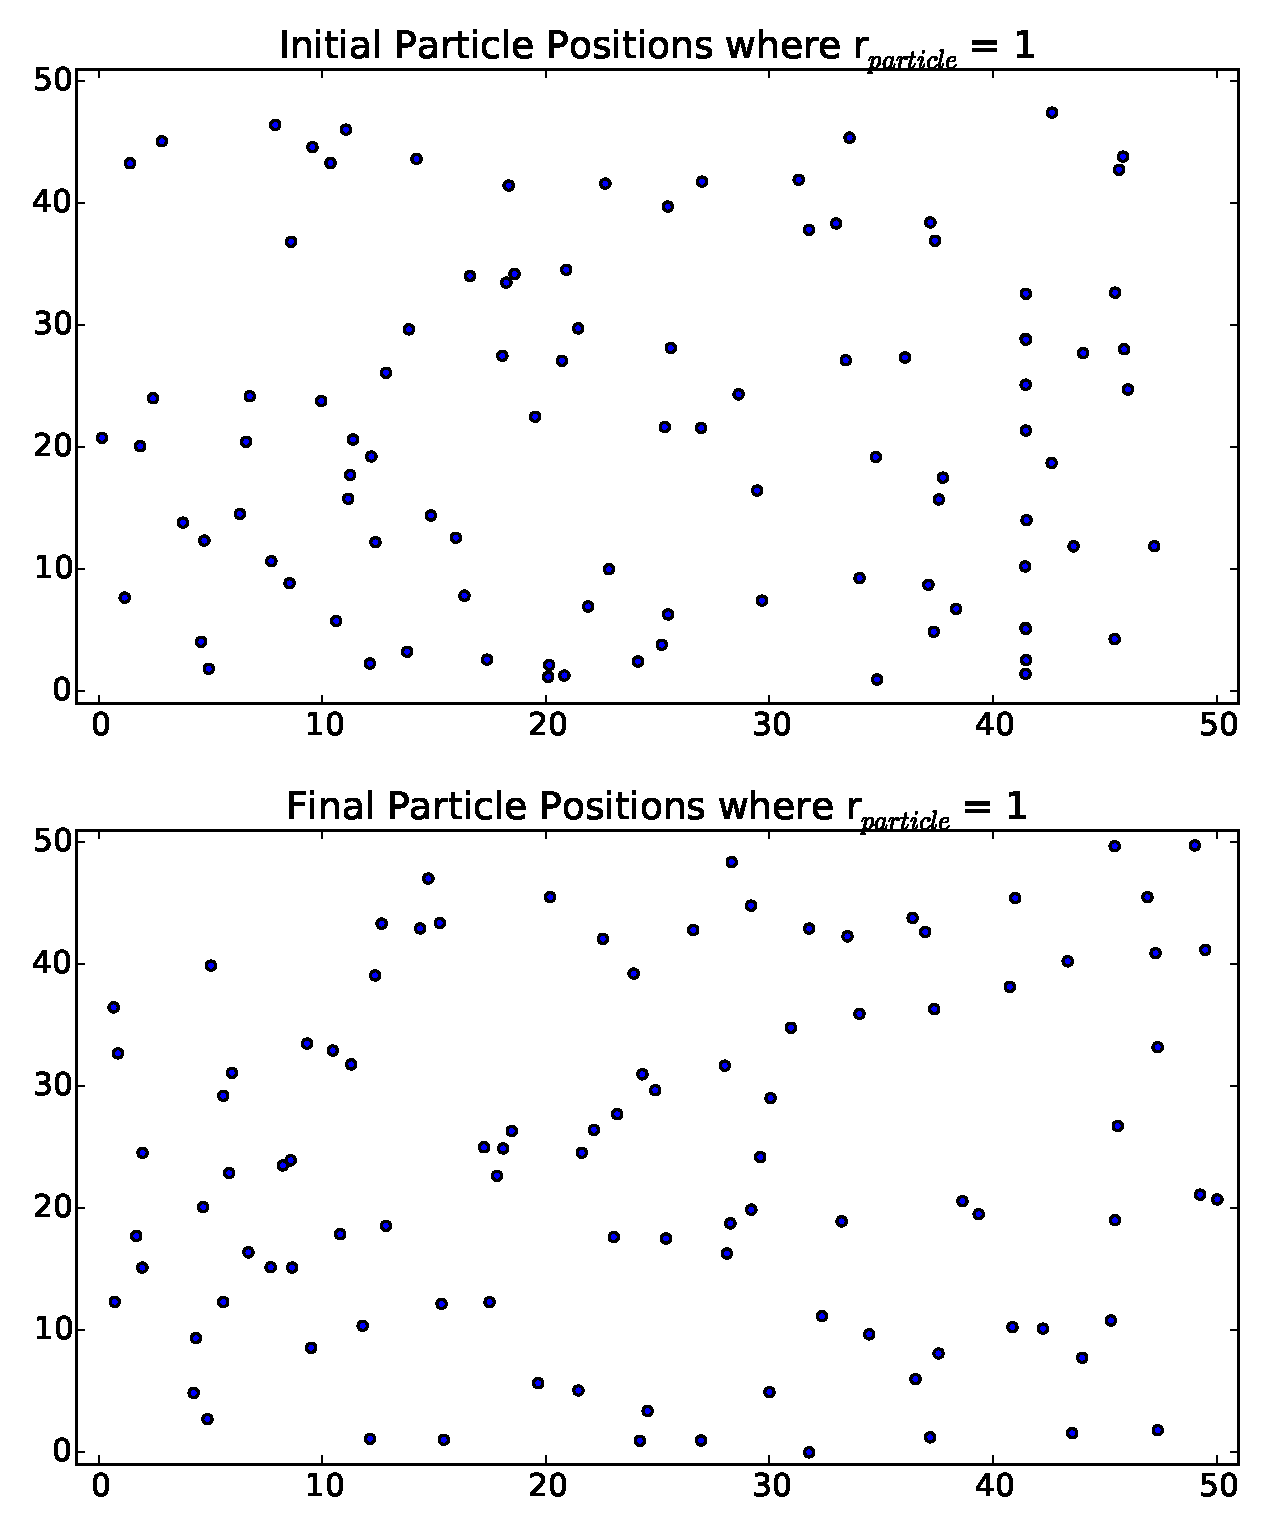
\includegraphics[width=1.0\textwidth]{pos_dist.eps}
    \caption{Initial and final particle positions.}
\end{figure}

%%%QUESTION 2 %%%

\section{Simulation Velocity and Energy Distributions}

\subsection{a}

As derived on the attached sheet (see Fleming 1), the 2D Maxwellian distributions for velocity and energy are 

$$ \frac{dN}{dv} = \frac{N m}{k_b T} v e^{\frac{-m v^2}{2 k_b T}} $$

and

$$ \frac{dN}{dE} = \frac{N}{k_b T}  e^{\frac{-E}{k_b T}} $$

respectively.

\subsection{b}

After running 10 simulations for a sufficient length of time, the velocity and energy distributions reached a steady state.  For both velocity $v$ and energy $E$, the average histogram of the ten simulations for $v$ and $E$ at the initial and final states of the simulation are shown in Figures 2 and 3 over plotted with the theoretical expectation discussed above in $2.a$.  As shown in the figures, there is good agreement between the simulation results and theory.

%Show Vel Dist
\begin{figure}[h!]
  \centering
    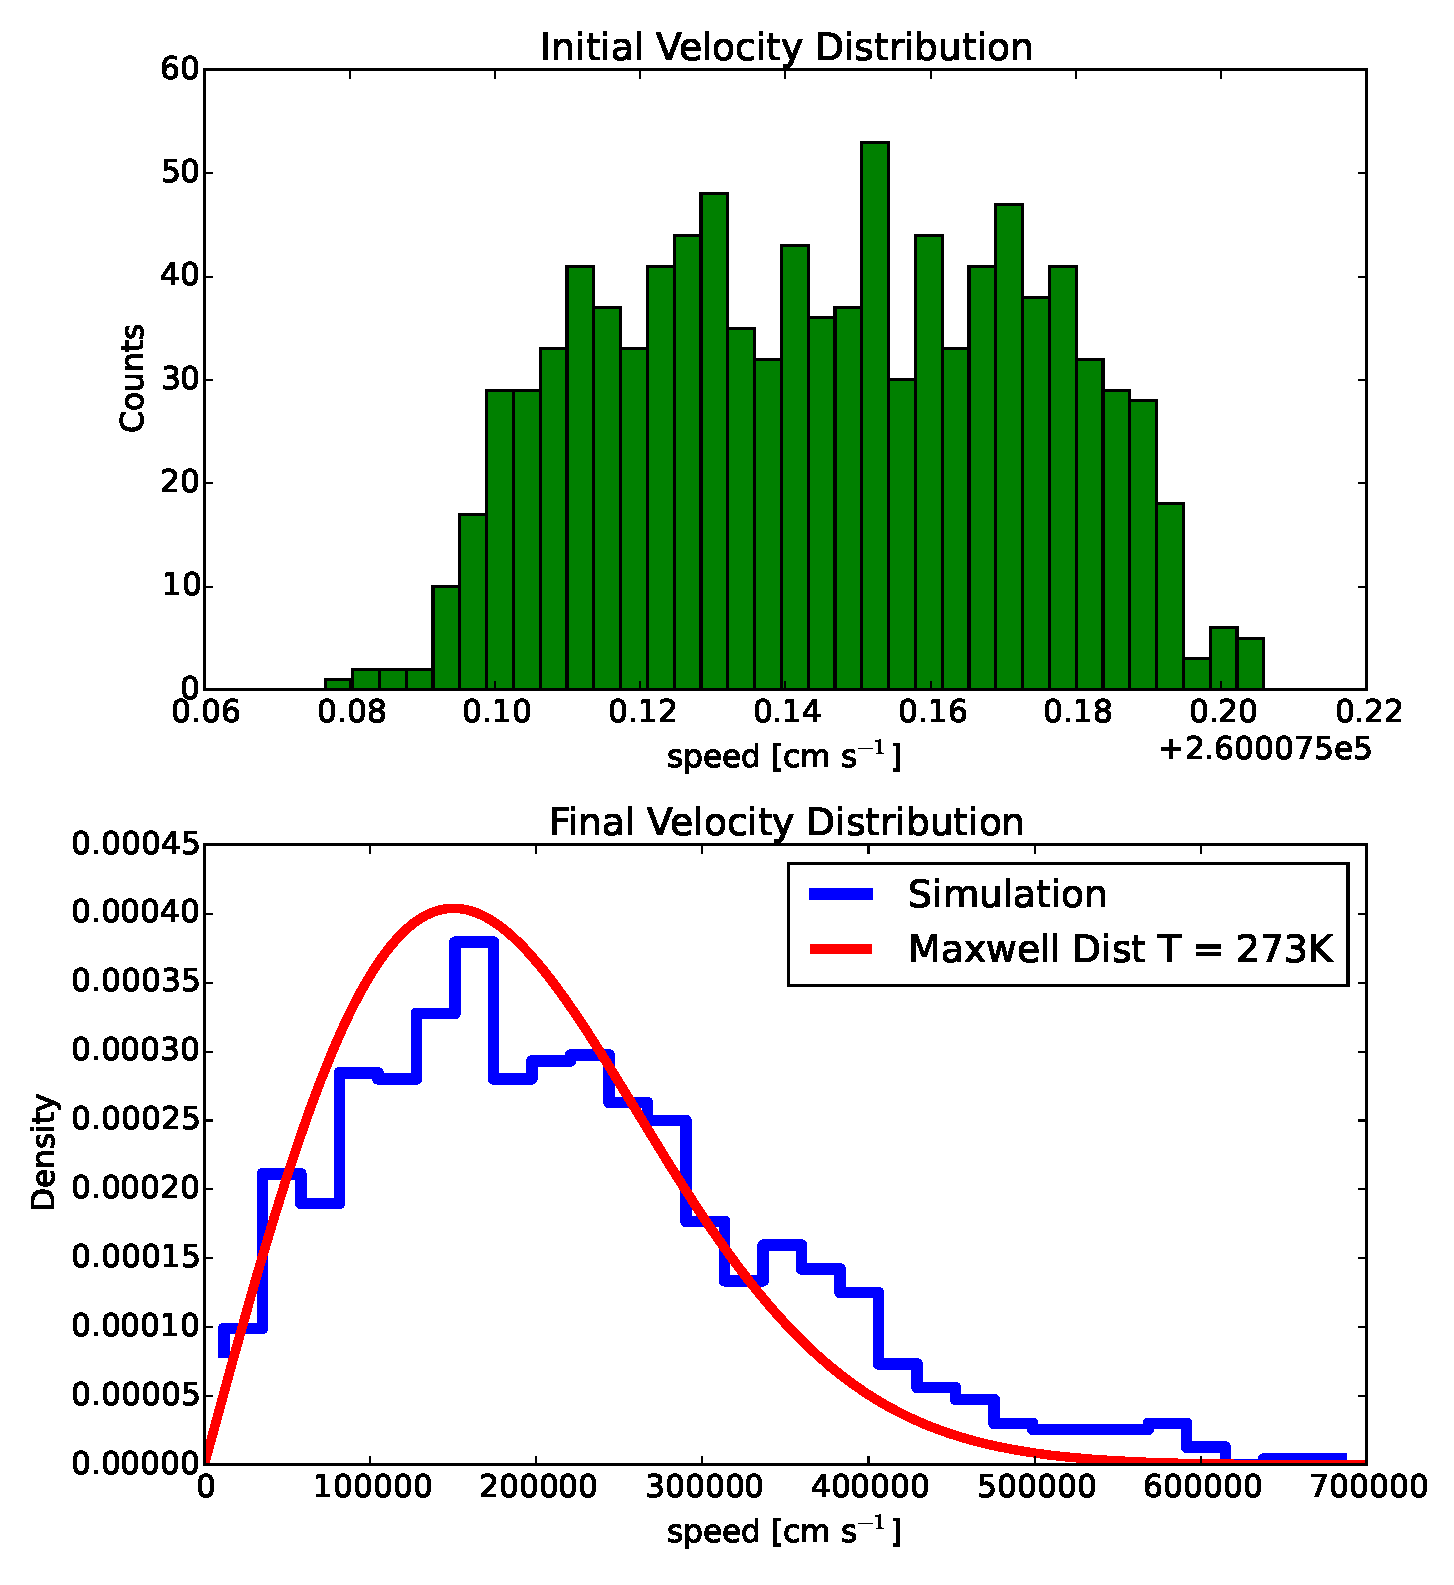
\includegraphics[width=1.0\textwidth]{vel_dist.eps}
    \caption{Simulated velocity distribution compared with theory.}
\end{figure}

%Show E Dist
\begin{figure}[h!]
  \centering
    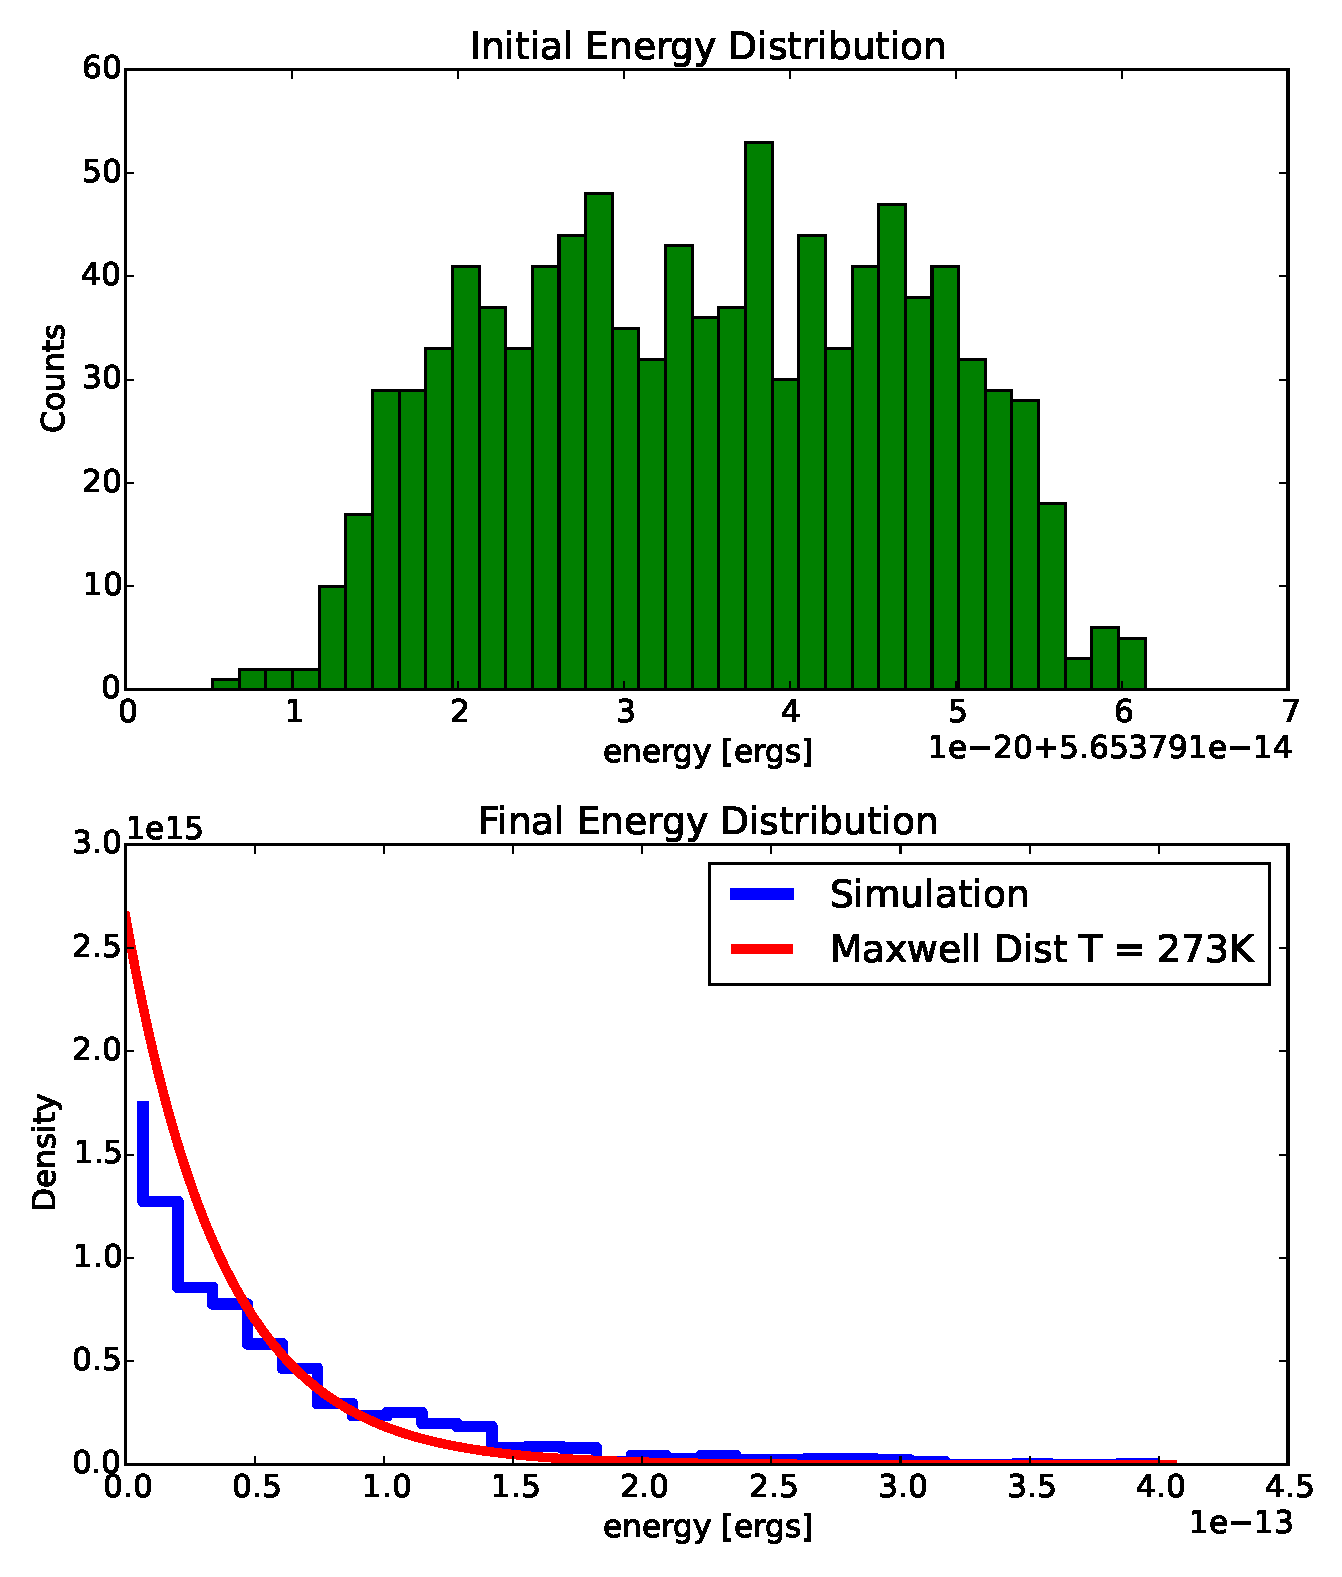
\includegraphics[width=1.0\textwidth]{energy_dist.eps}
    \caption{Simulated energy distribution compared with theory.}
\end{figure}

\subsection{c}

For one set of ten simulations, I made half of the particle masses 10 times larger.  The average histograms of $v$ and $E$ of the simulations are shown in Figures 4 and 5.  For the velocity distributions, it appears like the velocity distribution for the simulation with half of the particles being more massive is composed of two Maxwellians with a lower peak velocity than the standard simulation's distribution.  The mass dependence in $\frac{dN}{dv}$ causes a distribution to become tighter and centered around lower velocity values at a given temperature.  Since the temperature of the gas determines its energy and $E = \frac{1}{2}mv^2$, the more massive the particle, the slower it is.  Therefore it makes sense that the simulation with a higher average particle mass would have a tighter peak and at a lower velocity as is observed.  The two Maxwellian bumps in the distribution is likely due to the more massive particles kicking the lower mass particles to high velocity giving rise to the higher velocity bump.  For the energy distribution shown in Figure 5, we see that the two simulations are effectively identical.  This is because $\frac{dN}{dE}$ has no mass dependence as the temperature of the gas specifies the shape of the distribution.  The results in more massive particles moving more slowly and lighter particles moving faster at the same temperature to produce the same distribution shape.

%Show comp Vel Dist
\begin{figure}[h!]
  \centering
    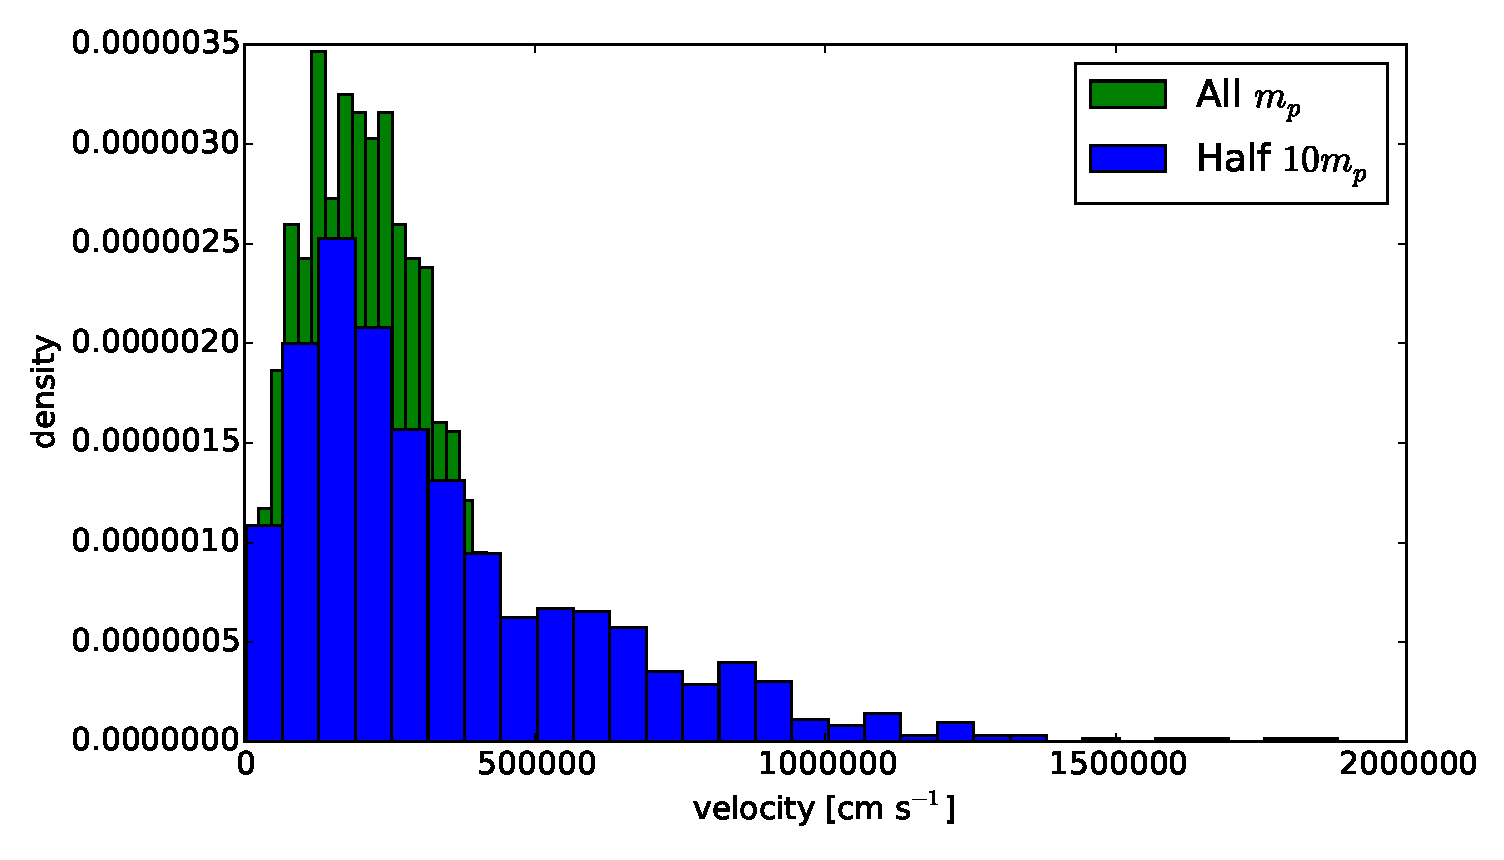
\includegraphics[width=1.0\textwidth]{vel_comp.eps}
    \caption{Comparison of the velocity distributions for all particle masses being $m_p$ (green) and for half being $10m_p$ (blue).}
\end{figure}

%Show comp energy Dist
\begin{figure}[h!]
  \centering
    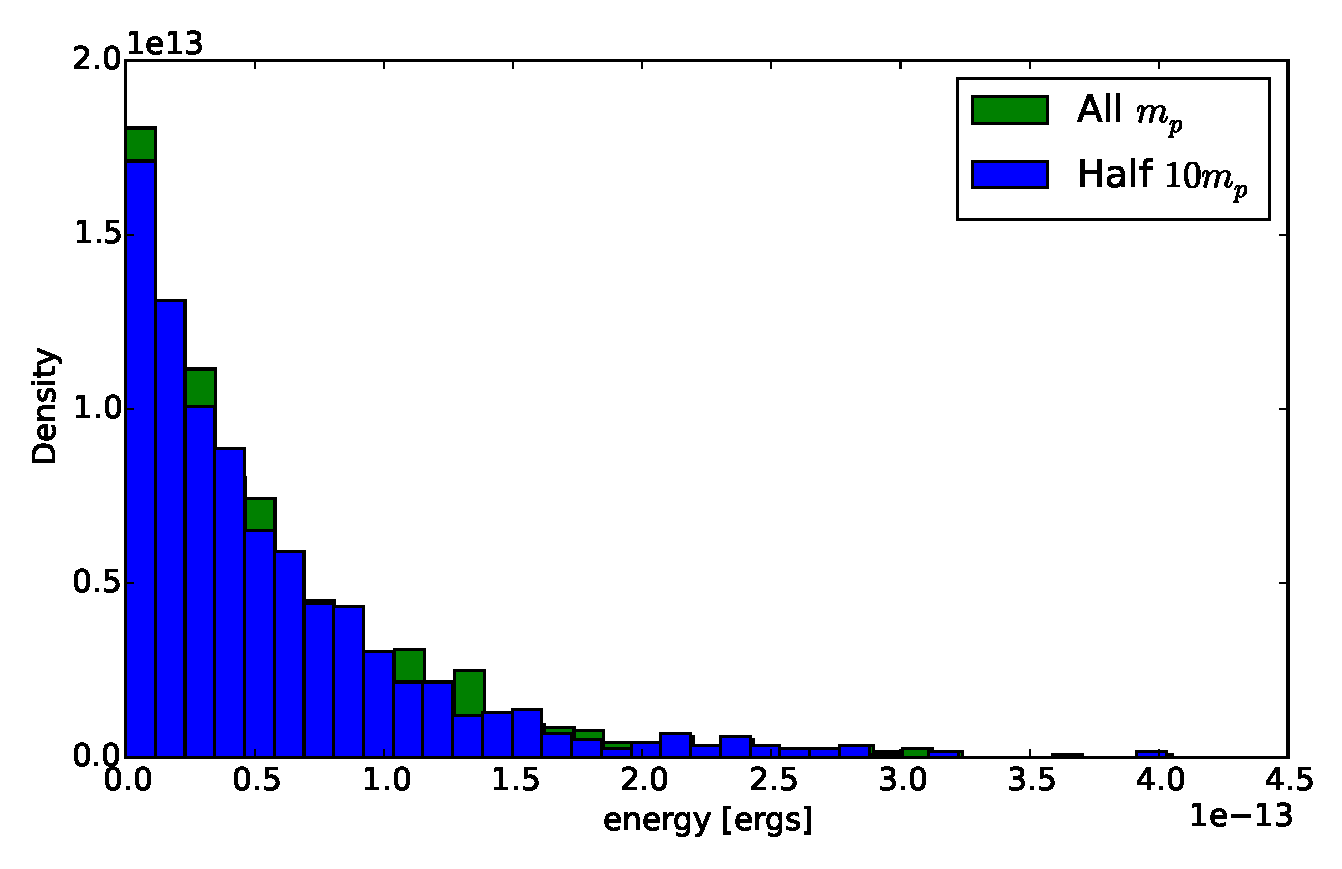
\includegraphics[width=1.0\textwidth]{energy_comp.eps}
    \caption{Comparison of the energy distributions for all particle masses being $m_p$ (green) and for half being $10m_p$ (blue).}
\end{figure}

%%% QUESTION 3 %%%

\section{Relaxation Timescale}





%%% QUESTION 4 %%%

\section{Ideal Gas Law}

The simulation ran for several values of both number density $n$ and temperature $T$ to see if the ideal gas law $P=nk_bT$ held.  For each $(n,T)$ pair, the simulation outputted the pressure computed by determining the average force on a wall due to incident particles (for a more complete discussion see the "Pressure" section).  These values were then plotted vs. the ideal gas law in Figure 6 to see if it indeed held for the simulations.  Within some small random scatter due to initial conditions, the results of the simulation matched the ideal gas law quite well within a factor of 2 or so.

%Show P=nkT
\begin{figure}[h!]
  \centering
    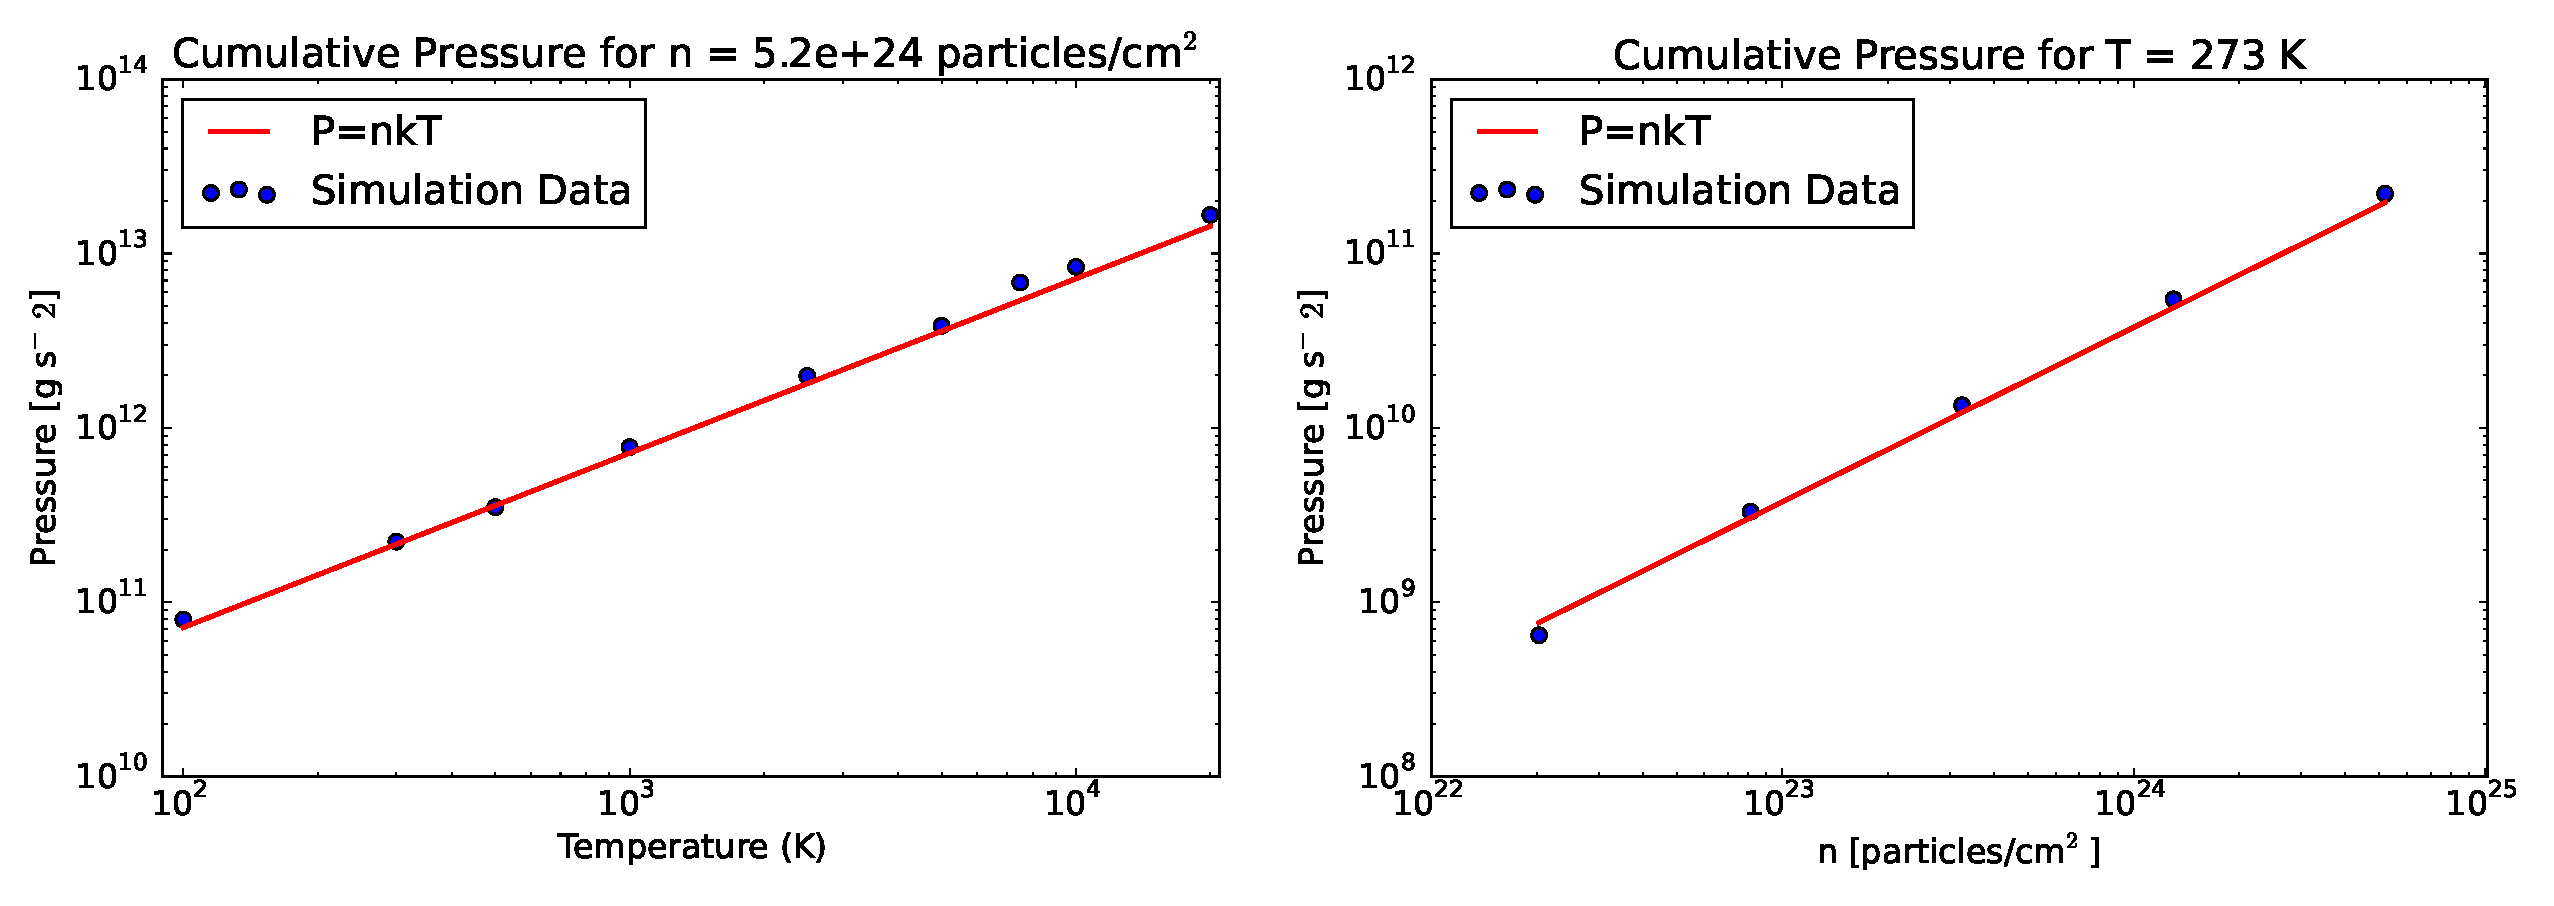
\includegraphics[width=1.0\textwidth]{pv_nrt.eps}
    \caption{Comparison of simulation results with the Ideal Gas Law.}
\end{figure}


\end{document}